
%(BEGIN_QUESTION)
% Copyright 2007, Tony R. Kuphaldt, released under the Creative Commons Attribution License (v 1.0)
% This means you may do almost anything with this work of mine, so long as you give me proper credit

A {\it current mirror} circuit may be thought of as a kind of control system.  Identify the {\it process variable} (PV), the {\it setpoint} (SP), the {\it output}, and the {\it loads} as they apply to a current mirror circuit:

$$\includegraphics[width=15.5cm]{i01735x01.eps}$$

Now, consider this circuit modification, and how it may be thought of as a {\it ratio} control system.  Identify what the ``ratio'' is, and what determines its value:

$$\includegraphics[width=15.5cm]{i01735x02.eps}$$

\vskip 20pt \vbox{\hrule \hbox{\strut \vrule{} {\bf Suggestions for Socratic discussion} \vrule} \hrule}

\begin{itemize}
\item{} A good problem-solving technique to apply here is assigning numerical values to the components (resistors).  For example, you might imagine a case where $R_1 = R_2$, just to prove to yourself how the circuit works, then after that imagine a case where $R_1 \neq R_2$.
\item{} Write an equation solving for the ``process variable'' current given $R_1$ and $R_2$ resistor values and the ``setpoint'' current.
\item{} Explain what will happen in this circuit if $R_{prg}$ fails open.
\item{} Explain what will happen in this circuit if $R_{prg}$ fails shorted.
\item{} Explain what will happen in this circuit if $R_{load}$ fails open.
\item{} Explain what will happen in this circuit if $R_{load}$ fails shorted.
\item{} Explain what will happen in the lower circuit if $R_1$ fails open.
\item{} Explain what will happen in the lower circuit if $R_1$ fails shorted.
\item{} Explain what will happen in the lower circuit if $R_2$ fails open.
\item{} Explain what will happen in the lower circuit if $R_2$ fails shorted.
\end{itemize}

\underbar{file i01735}
%(END_QUESTION)





%(BEGIN_ANSWER)

\begin{itemize}
\item{} PV = load current
\item{} SP = ``program'' current (through $R_{prg}$)
\item{} Output = current to base of $Q_2$
\item{} Loads = $+V_{load}$, $R_{load}$
\end{itemize}

\vskip 10pt

If $V_{BE}$ for both transistors will be approximately the same ($\approx$ 0.7 V), the base terminals of both are common, and both resistors $R_1$ and $R_2$ are common at ground, then $V_{R1} \approx V_{R2}$.  This means $I_{prg} R_1 \approx I_{load} R_2$, therefore ${I_{load} \over I_{prg}} \approx {R_1 \over R_2}$.

%(END_ANSWER)





%(BEGIN_NOTES)


%INDEX% Electronics review: current mirror

%(END_NOTES)


